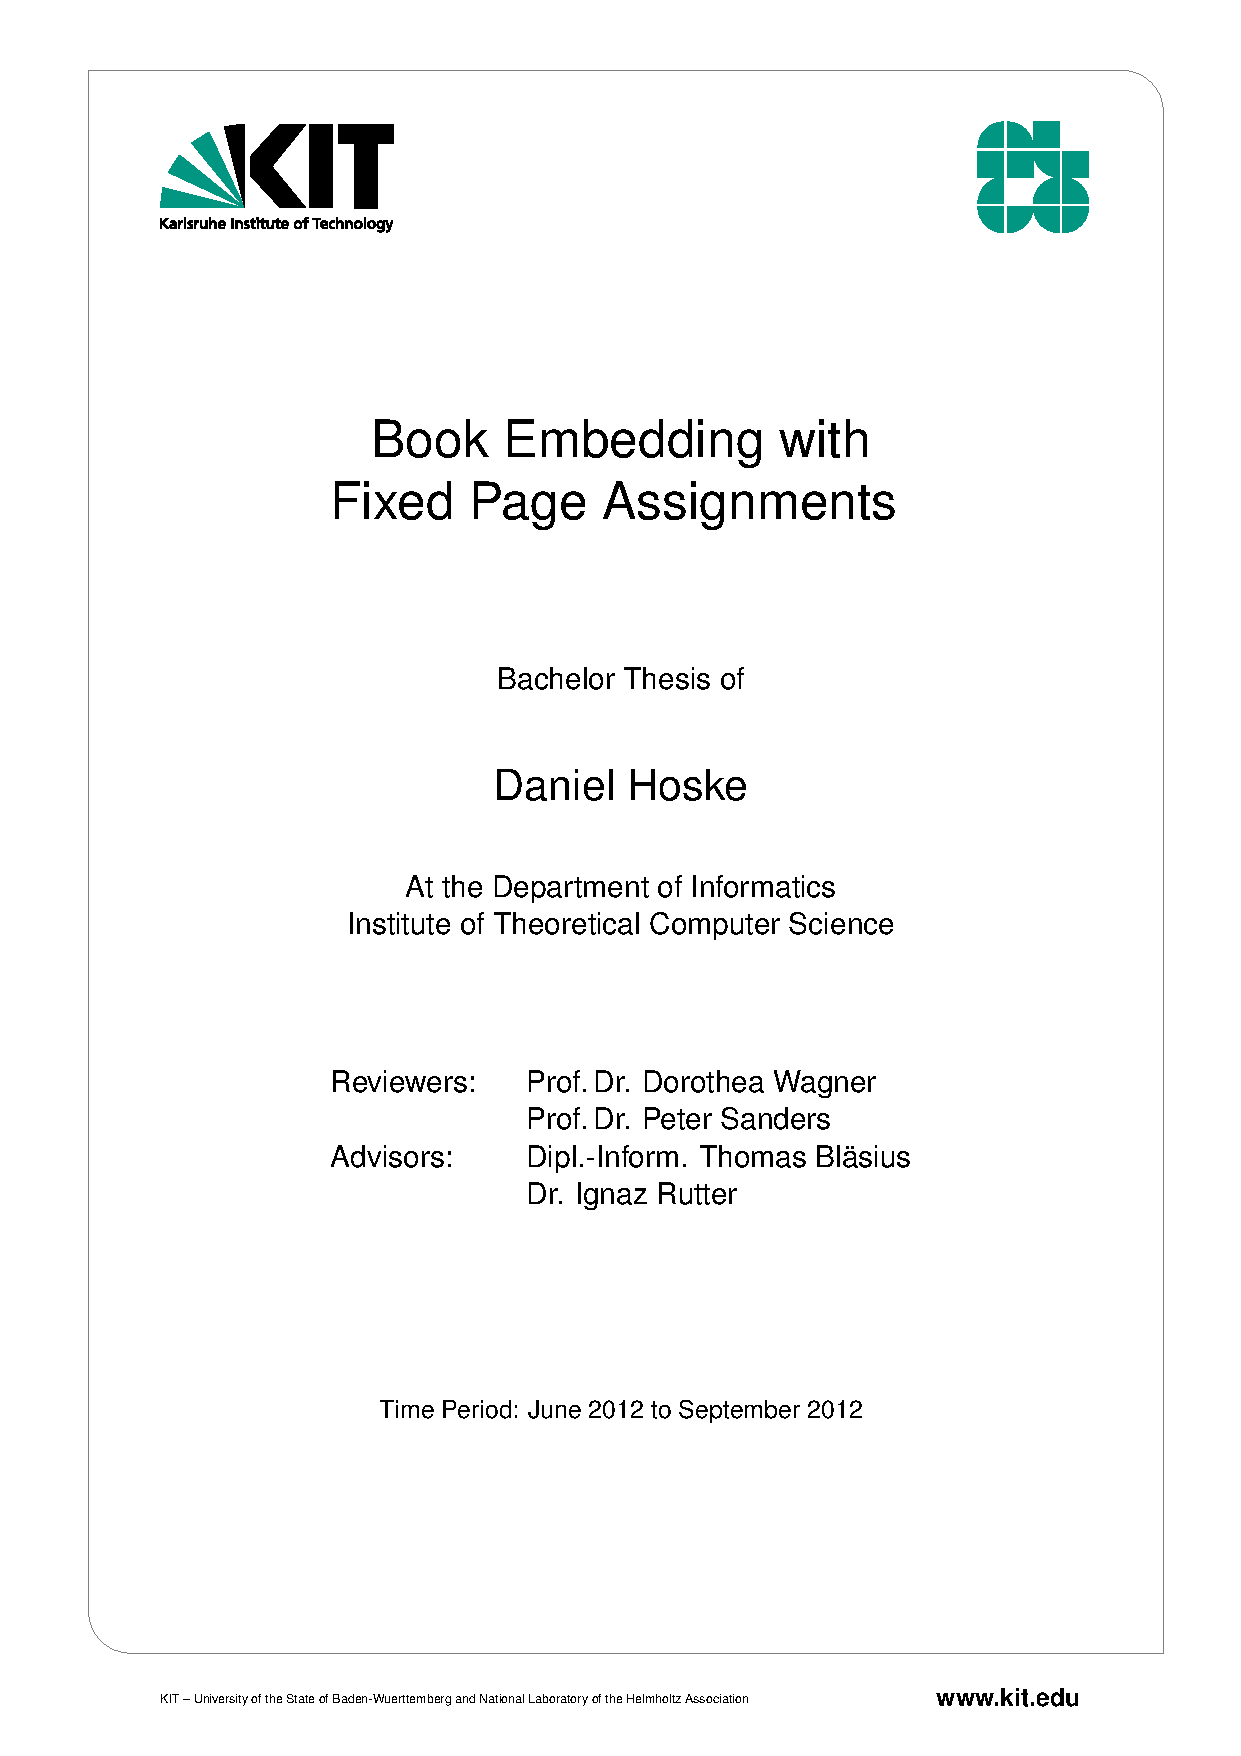
\includepdf{titlepage.pdf}
\cleardoublepage

\thispagestyle{plain}

\vspace*{\fill}

{\bf Statutory Declaration}

\vspace{0.25cm}

%I hereby declare that this document has been composed by myself and describes my own work unless %otherwise acknowledged in the text.

I hereby declare that this thesis is the result of my own work, that I used no other than
the indicated references and resources, that all the information that has been taken directly
or indirectly from other sources is indicated as such, and that I have regarded the statute of
the Karlsruhe Institute of Technology on securing good scientific practice in its currently
applicable version.

\vspace{1.5cm}

\makeatletter
\hspace{0.25cm} Karlsruhe, \@date
\makeatother

\vspace{2cm}

\newpage

%% -------------------
%% |   Abstract      |
%% -------------------
\infopage{Abstract}{%
A \emph{$k$-page book embedding} of a graph is a drawing of that graph in a book, with vertices along 
the book's \emph{spine}~(a straight~line) and edges in $k$~of the book's \emph{pages} (half~planes with the spine as boundary) such that the
edges do not cross. In this thesis we consider the problem of determining whether such a drawing exists  when the assignment of edges to
pages is predetermined. 

We start by showing that this problem is \NP-complete for an unbounded number of pages,
even if the edges on each page form a matching, and then solve some special cases. In the case of connected graphs on each page,
we provide a linear-time decision algorithm. When the graphs on each page are disjoint perfect matchings, we show that the graph has to be bipartite to be embeddable and give bipartite examples and counterexamples.

Following these results, we consider several variations of the problem. Firstly, if we constrain the vertex orders on the spine by a \PQ-tree only containing \Q-nodes as inner nodes, embeddability can be decided in quadratic time. Secondly, we alter the embedding problem by taking multiple spines~(parallel lines) in the plane
and associating every vertex with a spine the vertex has to be drawn on. 
Additionally, edges must be drawn between consecutive spines, above the
topmost spine or below the bottommost spine.
We show that this variation is equivalent to
a special case of the 2-page book embedding problem with
fixed page assignments where the vertex order is constrained
by a \PQ-tree only containing \PT-nodes as inner nodes.

At the end we outline the most important open problems for book embedding with
fixed page assignments and provide some suggestions on how to approach them.}

\selectlanguage{ngerman}
\infopage{Deutsche Zusammenfassung}{%
Eine \emph{$k$-Seiten Bucheinbettung} eines Graphens ist eine Zeichnung dieses Graphens
in einem Buch mit Knoten auf dem \emph{Buchrücken} (einer Geraden) und Kanten in~$k$ der \emph{Seiten} des Buches (Halbebenen mit dem Buchrücken als Rand). Dabei dürfen sich Kanten nicht kreuzen.
In dieser Arbeit betrachten wir das Problem, die Existenz einer solchen Zeichnung zu prüfen, wenn
die Zuordnung von Kanten zu Seiten fest ist.

Wir beginnen damit, die \NP-Vollständigkeit des Bucheinbettungsproblems für eine unbeschränkte Anzahl von Seiten
zu zeigen. Das Problem bleibt selbst dann \NP-vollständig, wenn die Graphen auf den Seiten Matchings sind.
Danach lösen wir einige Spezialfälle des Problems.

Zunächst geben wir für den Fall zusammenhängender Graphen auf den Seiten einen Linearzeitalgorithmus an.

Danach fordern wir, dass die Graphen auf den Seiten disjunkte perfekte Matchings
bilden. Einbettbare Graphen müssen in diesem Fall bipartit sein und wir konstruieren
bipartite Beispiele und Gegenbeispiele.

Nach diesen Spezialfällen betrachten wir verschiedene Varianten des Bucheinbettungsproblems. Zuerst wird die Ordnung der Knoten auf dem Buchrücken mittels eines \PQ-Baumes eingeschränkt, der nur \Q-Knoten
als innere Knoten hat. In diesem Fall ist Einbettbarkeit in quadratischer Zeit entscheidbar.

Anschließend betrachten wir mehrere Buchrücken (parallele Geraden) in der Ebene und ordnen
jeden Knoten einem dieser Buchrücken zu, auf dem er gezeichnet werden muss. Des Weiteren
sollen Kanten in dieser Variante zwischen den Buchrücken, oberhalb des obersten Buchrückens und
unterhalb des untersten Buchrückens gezeichnet werden. Diese Variante ist äquivalent
zu einem Spezialfall von 2-seitiger Bucheinbettung, wobei die Knotenordnung zusätzlich durch
einen \PQ-Baum beschränkt wird, der nur \PT-Knoten als innere Knoten hat.

Abschließend skizzieren wir die wichtigsten offenen Probleme für Bucheinbettungen mit fester Kantenzuordnung und
bestimmen einige Ansatzpunkte für deren Lösung.}
\selectlanguage{english}

\infopage{Acknowledgements}{%
I would like to express my deepest gratitude to my advisors Dr.~Ignaz Rutter and Dipl.-Inform.~Thomas Bläsius for their continued support, guidance, advice as well as for the insightful discussions	I had with them and to Prof.~Dorothea Wagner for giving me the chance of writing this thesis at her institute. Special thanks also go to every other proofreader of this thesis and anyone else who supported me during its writing in any shape or form.}

\cleardoublepage
%% -------------------
%% |   Directories   |
%% -------------------

\tableofcontents
\blankpage

\markboth{contents}{}
